\chapter{Teoremas de Existencia y Unicidad}



\subsection{Introducción}

\begin{quote}

 
 <<El determinismo es una doctrina filosófica que sostiene que todo acontecimiento físico, incluyendo el pensamiento y acciones humanas, está causalmente determinado por la irrompible cadena causa-consecuencia, y por tanto, el estado actual determina en algún sentido el futuro...En física, el determinismo sobre las leyes físicas fue dominante durante siglos, siendo algunos de sus principales defensores Pierre Simon Laplace y Albert Einstein.>>
 
<<Podemos mirar el estado presente del universo como el efecto del pasado y la causa de su futuro. Se podría condensar un intelecto que en cualquier momento dado sabría todas las fuerzas que animan la naturaleza y las posiciones de los seres que la componen. Si este intelecto fuera lo suficientemente vasto para someter los datos al análisis, podría condensarse en una simple fórmula de movimiento de los grandes cuerpos del universo y del átomo más ligero; para tal intelecto nada podría ser incierto y el futuro, así como el pasado, estaría frente sus ojos>>

\end{quote}
\begin{flushright}
Laplace, citado en \cite{ wiki:determinismo} \cite{Mazzo}
\end{flushright}


La ciencia se vale de estructuras matemáticas para describir a traves de modelos la evolución de sistemas reales. Usualmente esas estructuras son ecuaciones (diferenciales) donde el tiempo es una de sus variables. Conocer el estado actual de un sistema (las posiciones que menciona Laplace) es conocer las condiciones iniciales. Mientras que las ecuaciones en si mismas se derivan de  las fuerzas que animan la naturaleza.  Así, para que la matemática colabore con la filosofía determinista, debería ella misma plantear problemas deterministas.  En ese sentido, hablando específicamente de ecuaciones diferenciales, para que podamos decir que un PVI sea determinista, el problema debería tener solución (existencia de soluciones), caso contrario este PVI no produciría ninguna predicción del futuro. Pero también esta solución debería ser única (unicidad de soluciones), porque de no ser así, el problema produciría múltiples predicciones y por tanto el estado actual 
no determinaría el futuro. Un problema que satisfaga estas condiciones lo denominaremos \emph{bien planteado}\footnote{Es común en la literatura requerir, además de la existencia y unicidad, la estabilidad para hablar de problema bien planteado} . 

Por lo expuesto, es de trascendencia para la ciencia en general que se pueda establecer que los problemas matemáticos que modelizan problemas de estas ciencias sean bien planteados. Este es el propósito de este capítulo.


Para nuestra sorpresa, PVIs sin ningun problema aparente a la vista no son problemas bien planteados.

\begin{ejemplo}{} Considerar el siguiente PVI:
\[
  \left\{
 \begin{array}{ll}
    y'(x)&=y(x)^{2/3}\\
    y(0)&=0\\
 \end{array}
 \right.
\]

La ecuacion  s en variables separables. Deberíamos dividir por $y(x)$, pero notar antes de hacer ello que $y\equiv 0$ es solución. Supongamos $y(x)\neq 0$, una vez dividido
\[\frac{dy}{y^{2/3}}=dx\Rightarrow 3y^{1/3}=x+C\Rightarrow y(x)=\left(\frac{x}{3}+C\right)^3.\]
A pesar de la limitación original de que $y(x)\neq 0$, la expresión para $y(x)$ que hemos hallado es solución para todo $x\in\rr$. Notar que  $y(x)=0$ cuando $x=-C/3$. Sin embargo, el valor problemático $y=0$ nos trae aparejado un inesperado problema. Ocure  que la función $y_C(x):=\left(\frac{x}{3}+C\right)^3$ tiene derivada igual a cero en $x=-C/3$. Esto implica que si $C_1<C_2$ entonces la función 
\[
  y_{C_1,C_2}(x):=
  \left\{
 \begin{array}{ll}
    y_{C_1}(x)&\hbox{ si } x\leq-C_2\\
    0         &\hbox{ si } x\in [C_1,C_2]\\
    y_{C_2}(x) &\hbox{ si } x\geq -C_1\\
  \end{array}
 \right.
\]
está bien definida y es diferenciable en $\rr$. Además de ello, cualquiera de estas funciones con $C_1\leq 0 \leq C_2$ resuelven el PVI.  De esta manera hemos encontrado un PVI con infinitas soluciones.
\end{ejemplo}

\begin{tabular}{m{6cm} m{6cm}}
\begin{minipage}{6cm}
  \lstinputlisting[language=Python]{scripts/no-unicidad.py}
\end{minipage}

&
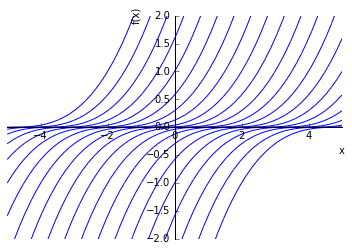
\includegraphics[scale=.4]{imagenes/no-unicidad.png}
 \end{tabular}




\section{Sistemas de Ecuaciones Diferenciales}
\subsection{Definición y ejemplos}
Un \emph{sistema de ecuaciones diferenciales de primer orden} es un conjunto  de ecuaciones que relacionan una variable independiente, digamos $x$, un conjunto de variables dependientes, digamos $y_1(x),\ldots,y_n(x)$, y sus derivadas respecto a $x$. A las ecuaciones diferenciales con una incognita y una ecuación las denominaremos \emph{ecuaciones escalares}.

\begin{definicion} Un sistema de ecuaciones diferenciales es una conjunto de ecuaciones de la forma
\begin{equation}\label{eq:sist_ecua}
\left\{
\begin{split}
 \frac{dy_1}{dx}(x)&=f_1(x,y_1(x),\ldots,y_n(x))\\
  \frac{dy_2}{dx}(x)&=f_2(x,y_1(x),\ldots,y_n(x))\\
       &\,\,\vdots                                   \\
 \frac{dy_n}{dx}(x)&=f_n(x,y_1(x),\ldots,y_n(x))\\
\end{split}\right.,
\end{equation}
donde $f_j:[a,b]\times\rr^n\to\rr$, $j=1,\ldots,n$, son funciones.

Una manera alternativa y compacta de denotar un sistema se logra introduciendo las funciones $y=(y_1,\ldots,y_n)$  y $f=(f_1,\ldots,f_n)$. Entonces $y:[a,b]\to\rr^n$ es una función con valores en $\rr^n$ y $f:[a,b]\times \rr^n\to\rr^n$ es un campo vectorial dependiente de $x$. Con estas notaciones el sistema se escribe:
\begin{equation}\label{eq:sist_ecua_comp}
 y'(x)=f(x,y(x)).
\end{equation}

\end{definicion}






\begin{ejemplo} [Ecuación del péndulo]{} Si $x(t)$ es el ángulo que forma un péndulo, de longitud $l$, con la vertical en el tiempo $t$ y $v(t)=x'(t)$, entonces $x(t)$ y$v(t)$ deben satisfacer el siguiente sistema de  ecuaciones:
\begin{equation}\label{eq:sist_pend}
\left\{
\begin{split}
 x'(t)&=v(t)\\
  v'(t)&=-\frac{g}{l}\sen(x(t)).\\
\end{split}\right.
\end{equation}


\end{ejemplo}


\begin{ejemplo}[Sistemas de ecuaciones de Lotka-Volterra]{}
 En 1925 y 1926, Alfred J. Lotka y Vito Volterra respectivamente, introdujeron
 las \href{https://es.wikipedia.org/wiki/Ecuaciones_Lotka%E2%80%93Volterra}{ecuaciones de Lotka-Volterra}. \marginpar{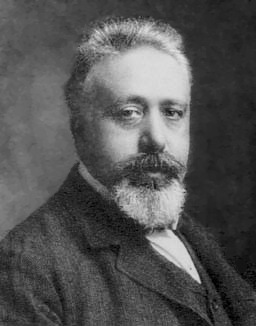
\includegraphics[scale=.28]{imagenes/Vito_Volterra.jpg}\\
 Vito Volterra (1860-1940)}  Se trata de un sistema de dos ecuaciones diferenciales de primer orden que se usan para describir dinámicas de sistemas biológicos en el que dos especies interactúan, una como presa y otra como depredador. Se definen como:
\begin{equation}\label{eq:lotka_volterra}
\left\{
\begin{split}
 x'(t) &= x(t) ( \alpha - \beta  y(t) )\\
  y'(t)&=-y(t)(\gamma-\delta x(t))\\
\end{split}\right.
\end{equation}
La variable $y$ representa el número de individuos de algún predador (por ejemplo, un lobo) y $x$ es el número de sus presas (por ejemplo, conejos), $t$ representa el tiempo; y  $\alpha,\beta,\gamma$ y $\delta$ son parámetros (positivos)

\end{ejemplo}


\subsection{Sistemas de ecuaciones y ecuaciones de orden superior}

\emph{Es posible convertir el sistema \eqref{eq:sist_ecua} de $n$-ecuaciones diferenciales de primer orden  en una ecuación escalar de orden $n$
\begin{equation}\label{eq:orden_n}
y^{(n)}=f(x,y,y',\ldots,y^{(n-1)}).
\end{equation}
y viceverza.}

Para justificar la aseveración anterior supongamos que $y=y(x)$ resuelven  \eqref{eq:orden_n} y escribamos:
\[y_1=y,\, y_2=y',\,y_3=y'',\ldots, y_{n}=y^{(n-1)}.\]
Entonces notar que
\begin{equation}\label{eq:sist_ecua_conv}
\left\{
\begin{array}{l l l}
 y_1'(x)&=y_2(x)\\
  y_2'(x)&=y_3(x)\\
       &\,\,\vdots\\
  y_{n-1}'(x)&=y_n(x)\\
 y_n'(x)&=f(x,y_1(x),\ldots,y_n(x))\\
\end{array}\right.,
\end{equation}

Reciprocamente, supongamos que $y_1,\ldots,y_n$ resuelven \eqref{eq:sist_ecua}. Por simplicidad vamos a suponer que las $f_j$ son independientes de $x$, el procedimiento general sigue las mismas líneas que el caso que discutimos aquí. Se toma $y=y_n$ (podríamos usar cualquier $y_j$, $j=1,\ldots,n$). Ahora derivamos sucesivamente $n$-veces respecto a $x$ la ecuación para $y_n$,  y reemplazamos cada derivada $y_j'$ por $f_j$ (vamos a omitir los argumentos de $f_j$ que son en todos los casos $(y_1,\ldots,y_n)$):

\[%\label{eq:sist_ecua_conv}
\begin{array}{c c c}
y_n'(x) =& f_n(y_1,\ldots,y_n) &\eqqcolon g_1(y_1,\ldots,y_n)\\
 y_n''(x)=&\sum\limits_{j=1}^n\frac{\partial f_n}{\partial y_j}f_j+
 & \eqqcolon g_2(y_1,\ldots,y_n)\\
  y_n'''(x)=&\sum\limits_{k,j=1}^n\frac{\partial^2 f_n}{\partial y_k \partial y_j}f_kf_j+
  \sum\limits_{k,j=1}^n\frac{\partial f_n}{\partial y_j}\frac{\partial f_j}{\partial y_k}f_k & \eqqcolon g_k(y_1,\ldots,y_n)\\
  &\,\,\vdots &\,\,\vdots \\
  y^{(n)}_n(x) =&\cdots & \eqqcolon g_n(y_1,\ldots,y_n)
  \\
\end{array}
\]
%\end{equation}
Las igualdades anteriores tienen la estructura $z=G(y)$, donde $y=(y_1,\ldots,y_n)$, $z=(y_n',y_n'',\ldots,y_n^{(n)})$ y $G=(y_1,\ldots,y_n)$. Si la función $G:\rr^n\to\rr^n$ es invertible y escribimos $H=G^{-1}$ entonces
\[y_n=H_n(z)=H_n(y_n',y_n'',\ldots,y_n^{(n)}).\]
La anterior es una ecuación escalar de orden $n$ para $y_n$. Por consiguiente hemos logrado reducir el sistema de $n$-ecuaciones a una ecuación de orden $n$. Observar que si resolvemos esta ecuación, encontrando $y_n$, podemos hallar el resto de las incognitas $y_j$, $j=1,\ldots,n-1$,  usando que $y_j=H_j(y_n',y_n'',\ldots,y_n^{(n)})$.


\begin{ejemplo}[Ecuaciones de Lotka-Volterra.]{} Reduzcamos las ecuaciones de Lotka-Volterra a una ecuación de orden 2 y luego revirtamos el camino.

La primera parte la resolvemos con Sympy:
\lstinputlisting[language=Python]{scripts/Sist-Ecua.py}
Resulta en
\begin{equation}\label{eq:lotka_escalar}\frac{d^{2}}{d t^{2}}  y{\left (t \right )- \frac{d}{d t} y{\left (t \right )} +
\left(- \alpha \gamma - \alpha\right) y{\left (t \right )} + \left(\beta \gamma + \beta\right) y^{2}{\left (t \right )} }=0
\end{equation}

El camino inverso es más sencillo. Llamamos $z=y'$. Usando las variables $y,z$ la ecuación \eqref{eq:lotka_escalar} se escribe
\[
 \left\{
 \begin{array}{ll}
    y'(t)&=v(t)\\
    v'(t)&=v+\left( \alpha \gamma + \alpha\right) y{\left (t \right )} - \left(\beta \gamma + \beta\right) y^{2}{\left (t \right )}
 \end{array}
 \right.
 \]

 No llegamos a la ecuación de partida. Hay que tener presente que una ecuación tiene diferentes representaciones en diferentes variables y que las variables que hemos elegido para el camino de vuelta $y,v$, no son las originales del problema $y,x$.


\end{ejemplo}


\section{Método de iteraciones de Picard}

En esta sección vamos a describir la estrategia que emplearemos para la demostración de la existencia de soluciones. El método que seguiremos fue ideado por \href{https://es.wikipedia.org/wiki/Charles_%C3%89mile_Picard}{Émile Picard} \marginpar{
    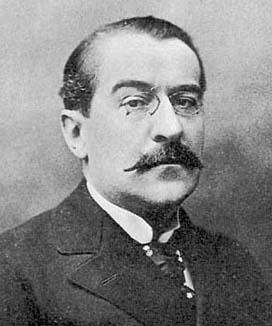
\includegraphics[scale=.3]{imagenes/Picard.jpg}\\
    Émile Picard (1856-1941)
}

Introducimos previamente algunas definiciones elementales.

\begin{definicion}
 Sea $\alpha$ una función  definida en un intervalo $[a,b]\subset \rr$ con valores en $\rr^n$, $n\geq 1$, tal que cada componete es una función integrable. Entonces, como es usual, escribimos
 \[\int_a^b\alpha(s)ds=\left(\int_a^b\alpha_1(s)ds,\ldots,\int_a^b\alpha_n(s)ds\right) \]
\end{definicion}

Es un ejercicio muy sencillo  demostrar que vales las propiedades elementales de las integrales, para esta extensión del concepto de integral a funciones con valores vectoriales. En particular vale el Teorema Fundamental del Cálculo: \emph{Si $\alpha$ es continuamente diferenciable entonces
\[ \int_a^b\alpha'(s)ds=\alpha(b)-\alpha(a).\]
}

Además vale la \emph{desigualdad triangular:} si $a<b$
\[\left\|\int_a^b \alpha(s)ds\right\|\leq \int_a^b \left\|\alpha(s)\right\|ds.\]
Nuestra intención es demostrar la existencia de soluciones de un PVI para el sistema de EDOs
\boxedeq{
\left\{
\begin{array}{ll}
 y'(x)&=f(x,y)\\
 y(x_0)&=y_0\\
\end{array}
\right. ,
}{eq:PVI_prin}

donde $f:\Omega \subset (a,b)\times \rr^n\to \rr^n$, $\Omega$ abierto, $y:(a,b)\to \rr^n$ (se debe satisfacer que $(x,y(x))\in \Omega$, para $x\in [a,b]$), $x_0\in (a,b)$
e $y_0\in\rr^n$ son dados con $(x_0,y_0)\in \Omega$.



Integremos la ecuación diferencial en un intervalo de extremos $x_0$ y $x$ y tomando en consideeración las condiciones iniciales obtenemos una nueva ecuación para $y(x)$,  en este caso una \href{https://es.wikipedia.org/wiki/Ecuaci%C3%B3n_integral}{ecuación integral} :

\boxedeq{
y(x)=y_0+\int_{x_0}^xf(t,y(t))dt.
}{eq:ecua_int}

Esta ecuación presenta una estructura muy particular. Podemos pensar el miembro derecho de \eqref{eq:ecua_int} como una trasformación (función) $T$ que lleva la función $y=y(x)$ en la función
\[
 T(y)(x):=y_0+\int_{x_0}^xf(t,y(t))dt.
\]
Pensando de esta manera  \eqref{eq:ecua_int} se escribe sencillamente
\[
 T(y)=y.
\]
Vale decir, la ecuación integral expresa el hecho que $T$ lleva a la función $y$ en si misma. Esto en matemática es conocido como un \href{https://es.wikipedia.org/wiki/M%C3%A9todo_del_punto_fijo}{punto fijo}. En análisis numérico los puntos fijos son utilizados para resolver ecuaciones algebraicas del tipo $h(x)=x$, donde $h:\rr\to\rr$. En aquel copntexto se ve que un procedimiento para aproximar soluciones es interar la función $h$, i.e. dado un $x_0$ cualquiera considerar la sucesión de \emph{aproximaciones sucesivas}
\[x_n=h(x_{n-1}),\quad n=1,2,\ldots.\]
El fundamento de proceder así es que si la sucesión $x_n$ converge a algún valor $x^*$ y si $h$ es continua entonces $x^*$ resuelve $h(x)=x$ pues
\begin{equation}
\label{eq:pto_fijo}h(x^*)=h\left(\lim_{n\to\infty} x_n\right)=\lim_{n\to\infty} h(x_n)=\lim_{n\to\infty} x_{n+1}=x^*.
\end{equation}

Vamos a proceder por analogía y proponer el siguiente proceso iterativo que genera las funciones $\varphi_k$, $k=0,1,\ldots$:

\boxedeq{
\left\{
\begin{array}{ll}
\varphi_0&=y_0\\
\varphi_{k+1}(x)&=y_0+\int_{x_0}^xf(t,\varphi_k(t))dt.\\
\end{array}
\right. .
}{eq:iter_picard}

Este proceso se denomina \emph{método de las aproximaciones sucesivas de Picard} y fué propuesto por E. Picard en  \cite{EmilePicard1893} y luego generalizado por \href{https://es.wikipedia.org/wiki/Ernst_Leonard_Lindel%C3%B6f}{Ernest Lindelöf}  en \cite{ErnestLindelof1894}. \marginpar{
    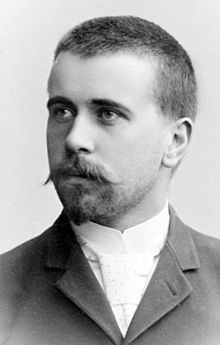
\includegraphics[scale=.3]{imagenes/Lindelof.jpg}\\
   Ernst L. Lindelöf (1870—1946)
}



Deberemos indagar por condiciones que nos aseguren que la sucesión $\varphi_k$ converja a una función $\varphi$ y que esta función $\varphi$ es solución del PVI. Antes de adentrarnos en los detalles de las demostraciones, constatemos que la idea funciona en algunos ejemplos sencillos.

\begin{ejemplo}{} Resolver
\[
 \left\{
 \begin{array}{ll}
 y'(x)&=y(x)\\
 y(0)&=y_0\\
 \end{array}
  \right. ,
\]
donde $y:\rr\to\rr$ e $y_0$ es un punto arbitrario de $\rr$.

Aplicando el método de picard:
\[
 \begin{array}{lll}
  \varphi_0(x)&=y_0 &\\
  \varphi_1(x) &= y_0+\int_{0}^x \varphi_0(t)dt &= y_0(1+x)\\
  \varphi_2(x) &= y_0+\int_{0}^x \varphi_1(t)dt &= y_0(1+x+\frac{x^2}{2})\\
               &\,\vdots                        &\,\vdots                 \\
  \varphi_k(x) &= y_0+\int_{0}^x \varphi_k(t)dt &= y_0(1+x+\cdots+\frac{x^k}{k!})\\
 \end{array}
\]
Se aprecia que en $\varphi_k$ aparecen las sumas parciales del desarrollo en serie de Taylor alrededor de $0$ de la función exponencial. Luego tenemos que $\varphi_k$ converge a $y_0e^x$ que es justamente la solución delm PVI propuesto.
\end{ejemplo}

Más ejemplos será tratados en la actividad práctica.

\section{\href{https://es.wikipedia.org/wiki/Teorema_del_punto_fijo_de_Banach}{Teorema de punto fijo Banach}}

\begin{definicion} Sea $(X,d)$ un espacio métrico completo. Una función $K:X\to X$ se denominará una contracción si existe un $\theta\in [0,1)$ tal que
\[d(K(x),K(y))\leq \theta d(x,y),\quad x,y\in X.\]
\end{definicion}

Dada una función $K:X\to X$ escribiremos
\[K^n(x)=\underbrace{K\left( K \left( K\cdots K(x)\cdots \right)\right)}_{n-\hbox{veces}}.\]
Cuando $n=0$ ponemos $K^0(x)=x$.

\begin{teorema}[Principio de contracción de Banach]{teo:banach}  Sea $(X,d)$ un espacio métrico completo y $K:X\to X$  una contracción. Entonces $K$ tiene un único punto fijo $x^*$. Además para todo $x$
\[d(K^n(x),x^*)\leq \frac{\theta^n}{1-\theta}d(K(x),x).\]
\end{teorema}\marginpar{
    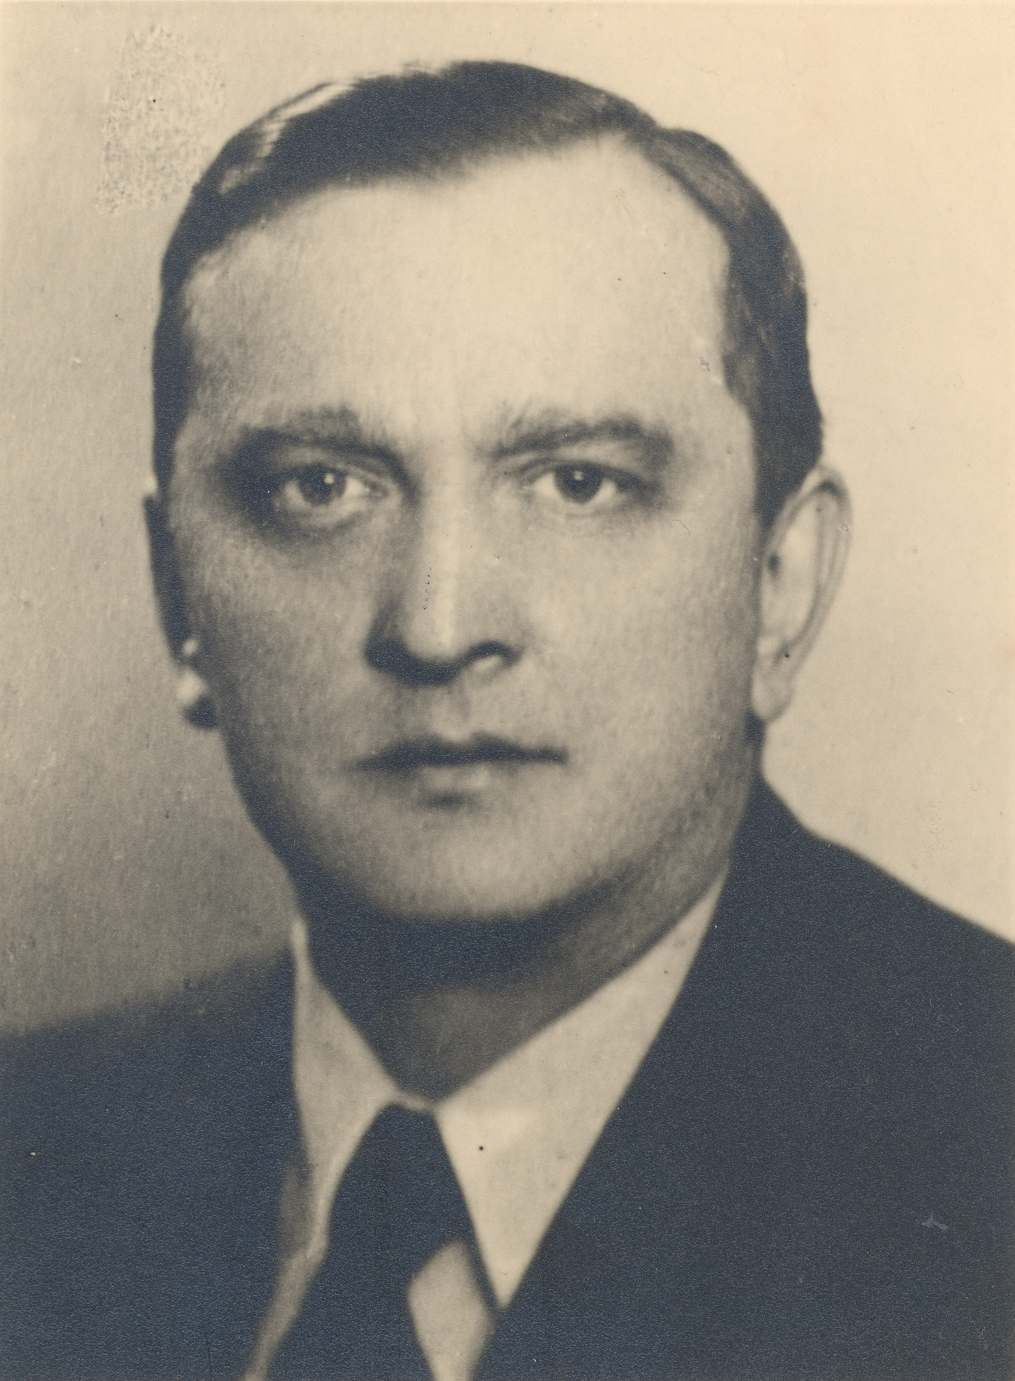
\includegraphics[scale=.3]{imagenes/banach.jpg}\\
   Stefan Banach (1892—1945)
}
\begin{proof} Sea $x\in X$ un punto arbitrario y definimos $x_n:=K^n(x)$. Entonces si $m<n$
\[
\begin{split}
 d(K^n(x),K^m(x))&\leq d(K^n(x),K^{n-1}(x))+\cdots+ d(K^{m+1}(x),K^m(x))\\
 &\leq \theta^{n-1} d(K(x),x)+\cdots + \theta^m d(K(x),x)\\
 &\leq \frac{\theta^m}{1-\theta}d(K(x),x)
 \end{split}
\]
Como $\theta<1$ vemos que si $m,n$ son suficientemente grandes podemos hacer que $ d(K^n(x),K^m(x))$ sea arbitrariamente chico. Hemos probado que la sucesión $K^n(x)$ es de Cauchy, de allí tiene límite, al que llamaremos $x^*$. Que $x^*$ es punto fijo se justifica como en \eqref{eq:pto_fijo} (notar que una contracción es continua).

Que el punto fijo es único, se deduce de suponer que existe otro $z^*$ y aplicar lque $K$ es contracción
\[d(x^* , z^*)=d(K(x^*) , K(z^*))\leq \theta d(x^* , z^*)<d(x^* , z^*).\]
Lo que es una contradicción.
\end{proof}

\begin{corolario}{cor:banach}  Sea $(X,d)$ un espacio métrico completo y $K:X\to X$ continua y $K^m$ contracción para algún $m\in\mathbb{N}$. Entonces $K$ tiene un único punto fijo $x^*$ y para todo $x\in X$ se tiene
\[ \lim_{n\to\infty} K^n(x)=x^*.\]
 \end{corolario}
 
 \begin{proof} Sea $x^*$ el único punto fijo de $K^m$ dado por el principio de contracción de Banach aplicado a $K^m$. Sean $x\in X$ y $0\leq r<m$. Consideremos las sucesiones $\{K^{km+r}(x)\}_{k\in\mathbb{N}}$. Tenemos $m$ de estas sucesiones, una para cada valor de $r=0,\ldots,m-1$. Todas ellas son subsucesiones de $\{K^n(x)\}_{n\in\mathbb{N}}$. Además 
  \[\bigcup_{r=0}^{m-1}\{K^{km+r}(x)\}_{k\in\mathbb{N}}=\{K^n(x)\}_{n\in\mathbb{N}}.\]
  Vamos a demostrar que estas $m$ subsucesiones convergen todas a $x^*$. Esto es facil consecuencia de que $K^m$ es contracción. Pues de ello obtenemos que $\left(K^{m}\right)^n(y)\to x^*$, cuando $n\to\infty$ para todo $y\in X$. Luego
  \[\lim_{k\to\infty}K^{km+r}(x)=\lim_{k\to\infty}\left(K^{m}\right)^k(K^r(x))=x^*.\]
  Esto establece que $ \lim_{n\to\infty} K^n(x)=x^*$.
  
  Veamos que $x^*$ es punto fijo de $K$. 
  \[K(x^*)=K\left(\lim_{n\to\infty} K^{n}(x)\right)=\lim_{n\to\infty} K\left( K^{n}(x)\right)
  =\lim_{n\to\infty}  K^{n+1}(x)=x^*.\]
  
  Para la unicidad, observar que un punto fijo de $K$ lo es de $K^m$. Cómo $K^m$ tiene un único punto fijo, lo mismo podemos afirmar de $K$.
  
 \end{proof}


\begin{definicion} Sea $f:\Omega \subset \rr^n\to \rr^m$. Diremos que $f$ es \emph{lipschitziana} (o que es una función Lipschitz) si existe una constante $K\geq 0$ tal que
\[\|f(x)-f(y)\|\leq L\|x-y\|,\quad \forall x,y\in \Omega .\]

Si $f:\Omega\subset\rr\times \rr^n\to\rr^m$, diremos que $f=f(t,x)$ es lipschitziana respecto a la segunda variable si existe  $K\geq 0$ tal que
\[\|f(t,x)-f(t,y)\|\leq L\|x-y\|,\quad \forall (t,x),(t,y)\in \Omega .\]
 
\end{definicion}



\begin{teorema}[Picard- Lindelöf]{teo:picard} Sean $x_0\in\rr$, $y_0\in\rr^n$ y $f:\Omega\to\rr^n$ continua y lipschitziana respecto a la segunda variable, donde $\Omega=I_a\times B_b$,  $I_a=[x_0-a,x_0+a]$ y $B_b=\{y\in\rr^n|\|y-y_0\|\leq b\}$. Como $\Omega$ es compacto y $f$ es continua, existe $M\geq 0$ tal que $\|f\|\leq M$. Entonces existe una única solución del PVI:
\[
 \left\{\begin{array}{ll}
	  y'(x)&=f(x,y(x)),\\
	  y(x_0)&=y_0\\         
        \end{array}
\right. ,
\]
en $I_{\delta}=(x_0-\delta,x_0+\delta)$ con $\delta:=\min\{a,b/M\}$.
 \end{teorema}

 \begin{proof}
 
 Definamos
\[X=C(I_{\delta},B_b):=\{\varphi| \varphi:I_a\to B_b\hbox{ continua }\}.\]
\begin{figure}[h]
  \begin{center}
\scalebox{.6} % Change this value to rescale the drawing.
{
\begin{pspicture}(0,-4.81)(10.393595,4.81)
\definecolor{color123b}{rgb}{0.9098039215686274,0.8431372549019608,0.8431372549019608}
\definecolor{color105b}{rgb}{0.8627450980392157,0.7607843137254902,0.7607843137254902}
\psellipse[linewidth=0.04,linestyle=dashed,dash=0.16cm 0.16cm,dimen=outer,fillstyle=solid,fillcolor=color105b](3.86,0.85)(0.44,1.3)
\psellipse[linewidth=0.04,linestyle=dashed,dash=0.16cm 0.16cm,dimen=outer](5.04,0.88)(0.4,1.29)
\psellipse[linewidth=0.04,linestyle=dashed,dash=0.16cm 0.16cm,dimen=outer,fillstyle=solid,fillcolor=color123b](6.07,0.86)(0.39,1.31)
\pspolygon[linewidth=0.04](0.0,-4.79)(0.04231884,2.37)(2.92,4.79)(2.86,-2.55)(2.88,-2.49)
\psbezier[linewidth=0.04](1.42,2.19)(0.96,2.05)(0.94,1.23)(0.92,0.93)(0.9,0.63)(0.92,-0.31)(1.42,-0.39)
\psbezier[linewidth=0.04,linestyle=dashed,dash=0.16cm 0.16cm](1.48,-0.41)(1.98,-0.27)(1.98,0.51)(1.98,0.93)(1.98,1.35)(1.9,2.27)(1.48,2.15)
\psline[linewidth=0.04cm](1.44,2.17)(7.1,2.15)
\psline[linewidth=0.04cm](1.44,-0.41)(7.02,-0.43)
\psellipse[linewidth=0.04,dimen=outer](7.0,0.86)(0.54,1.29)
\psline[linewidth=0.04cm,linestyle=dashed,dash=0.16cm 0.16cm](7.0,0.83)(1.46,0.81)
\psdots[dotsize=0.24](7.06,0.83)
\psdots[dotsize=0.12](1.5,0.83)
\psline[linewidth=0.04cm,arrowsize=0.05291667cm 2.0,arrowlength=1.4,arrowinset=0.4]{->}(1.5,0.77)(1.78,1.97)
\psline[linewidth=0.04cm,arrowsize=0.05291667cm 2.0,arrowlength=1.4,arrowinset=0.4]{->}(1.3,-1.77)(9.52,-1.71)
\usefont{T1}{ptm}{m}{n}
\rput(2.4290624,3.5){$\mathbb{R}^n$}
\usefont{T1}{ptm}{m}{n}
\rput(1.3590626,1.48){$b$}
\psline[linewidth=0.04cm,linestyle=dashed,dash=0.16cm 0.16cm](5.04,0.83)(5.0,-1.77)
\psline[linewidth=0.04cm,linestyle=dashed,dash=0.16cm 0.16cm](7.1,0.79)(7.1,-1.83)
\psline[linewidth=0.04cm,linestyle=dashed,dash=0.16cm 0.16cm](3.9,0.87)(3.86,-1.79)
\usefont{T1}{ptm}{m}{n}
\rput(5.0590625,-1.96){$x_0$}
\usefont{T1}{ptm}{m}{n}
\rput(6,-1.96){$x_0+\delta$}
\usefont{T1}{ptm}{m}{n}
\rput(3.8490624,-1.96){$x_0-\delta$}
\usefont{T1}{ptm}{m}{n}
\rput(1.5590626,0.52){$y_0$}
\psbezier[linewidth=0.04,arrowsize=0.05291667cm 2.0,arrowlength=1.4,arrowinset=0.4]{->}(6.4,3.39)(5.6,3.05)(6.6,2.49)(5.52,1.77)
\usefont{T1}{ptm}{m}{n}
\rput(6.4590626,3.42){$\Omega$}
\usefont{T1}{ptm}{m}{n}
\rput(9.049064,-1.48){$\mathbb{R}$}
\psline[linewidth=0.04cm,linestyle=dashed,dash=0.16cm 0.16cm](6.06,0.79)(6.08,-1.71)
\usefont{T1}{ptm}{m}{n}
\rput(7.2690625,-1.94){$x_0+a$}
\psbezier[linewidth=0.04,arrowsize=0.05291667cm 2.0,arrowlength=1.4,arrowinset=0.4]{->}(4.36,2.51)(4.5,1.53)(5.48,2.21)(5.12,0.95)
\psdots[dotsize=0.2](5.06,0.79)
\usefont{T1}{ptm}{m}{n}
\rput(4.2745314,2.78){$(x_0,y_0)$}
\end{pspicture} 
}
 \caption{Conjunto $I_{\delta}\times B_b$}\label{fig:exi_uni}
  \end{center}
\end{figure}
\begin{ejercicio} La función
\[d(\varphi_1,\varphi_2):=\max\left\{\|\varphi_1(x)-\varphi_2(x)\| \,\big| x\in I_{\delta}\right\}\]
  define una métrica sobre el conjunto $X$ y con esta métrica $(X,d)$ es completo. 
\end{ejercicio}

Para $\varphi\in X$, definamos una nueva función $K(\varphi)$ por:
\[K(\varphi)(x)=y_0+\int_{x_0}^xf(t,\varphi(t))dt.\]
\noindent\textbf{Afirmación 1:} $K:X\to X$. 

En efecto, si $x\geq x_0$ y $x\in I_{\delta}$ (si $x\leq x_0$ queda como ejercicio)
\[\|K(\varphi)(x)-y_0\|\leq \int_{x_0}^x\|f(t,\varphi(t))\|dt\leq M|x-x_0|\leq b.\]
Esto muestra que $K(\varphi):I_{\delta}\to B_b$. 

La continuad se establece del siguiente modo. Si $x_1<x_2$
\[
\|K(\varphi)(x_1)-K(\varphi)(x_2)\|\leq \int_{x_1}^{x_2}\|f(t,\varphi(t))\|dt\leq M|x_1-x_2|.\]

Lo que implica la continuidad. Entonces $K(\varphi)\in X$. 

\noindent\textbf{Afirmación 2:} $K^m$ es  contracción para $m$ suficientemente grande. 

La afirmación es consecuencia de la siguiente desigualdad, para $\varphi_1,\varphi_2\in X$ y $x\in I_{\delta}$
\[\|K^m(\varphi_1)(x)-K^m(\varphi)(x)\|\leq \frac{L^m|x-x_0|^m}{m!}d(\varphi_1,\varphi_2).\]
La prueba procede por induccón sobre $m$. Cuando $m=0$ es inmediata. Supuesta válida la desigualdad para $m$ vemos que (otra vez asumimos $x_0\leq x$)

\[
  \begin{split}
    \|K^{m+1}(\varphi_1)(x)&-K^{m+1}(\varphi)(x)\|=   \|K\left(K^{m}(\varphi_1)\right)(x)-K\left(K^{m}(\varphi)\right)(x)\|\\
    &=\left\|   
    \int_{x_0}^{x} f(t,K^m(\varphi_1)(t))- f(t,K^m(\varphi_2)(t)) dt
        \right\|\\
     &\leq    
    \int_{x_0}^{x} \left\|f(t,K^m(\varphi_1)(t))- f(t,K^m(\varphi_2)(t))\right\| dt\\
    &\leq     L\int_{x_0}^{x} \left\|K^m(\varphi_1)(t)- K^m(\varphi_2)(t))\right\| dt\\
    &\leq  \frac{L^{m+1}}{m!}d(\varphi_1,\varphi_2) \int_{x_0}^{x}  |t-x_0|^m dt\\
    &=\frac{L^{m+1}|x-x_0|^{m+1}}{(m+1)!}d(\varphi_1,\varphi_2)
  \end{split}
\]

Notar que $L^m|x-x_0|^m/m!$ es el valor absoluto del término general de la serie de Taylor de $e^{Lx}$ alrededor de $x_0$.Como esta serie tiene radio de convergencia infinito, el término general tiende a cero. Por consiguiente existe $m$ suficientemente grande para que $L^m|x-x_0|^m/m!<1$. Para este $m$, $K^m$ será contracción. Luego, por el Corolario \ref{cor:banach},  deducimos que $K$ tiene un único punto fijo. Vale decir que existe $y\in X$ con
\[
 y(x)=y_0+\int_{x_0}^xf(t,y(t))dt.
\]
Notar que $y(x_0)=y_0$, i.e. $y$ satisface la condición inicial. Por el teorema fundamental del cálculo $y'(x)=f(x,y(x))$, i.e. $y$ satisface la ecuación y por tanto, finalmente, es solución del PVI.\end{proof}


\begin{corolario}{} Sea $\Omega$ abierto de $\rr\times \rr^n$ y $f:\Omega\to\rr^n$ continua con $\partial f_j/\partial y_k)$ tambien continuas $j,k=1,\ldots,n$. Entonces para todo $(x_0,y_0)\in\Omega$ existe un entorno $V=[x_0-\delta,x_0+\delta]\times B_b(y_0)$ tal que el PVI
 \[
 \left\{\begin{array}{ll}
	  y'(x)&=f(x,y(x)),\\
	  y(x_0)&=y_0\\         
        \end{array}
\right. ,
\]
tiene solución única en $[x_0-\delta,x_0+\delta]$. Además el gráfico de esta solución está contenido en $V$..
\end{corolario}

\begin{proof} Sea $(x_0,y_0)\in\Omega$ arbitrario. Como $\Omega$ es abierto, existen $a,b>0$ tal que $[x_0-a,x_0+a]\times B_b(y_0)\subset \Omega$. Como $\partial f_j/\partial y_k)$ son continuas y $V$ es compacto, tenemos que existe $M>0$ con $|\partial f_j/\partial y_k)|\leq M$ en $V$, $j,k=1,\ldots,n$. El Teorema del valor medio para funciones en varias variables implica que existe una constante $C>0$ tal que si $(t,x),(t,z)\in V$
\[\|f(t,x)-f(t,z)\|\leq C M\|x-z\|.\]
i.e. $f$ es Lipschitziana respecto a la segunda variable en $V$. La conclusión del Corolario sigue del Teorema de Picard- Lindelöf. 
\end{proof}


   
\nocite{JorgeSotomayor513}.


% 
% 
%   \bibliographystyle{apalike}
%   \bibliography{diferenciales_ecuaciones,diferenciales_ecuaciones_sim}
